%%%%%%%%%%%%%%%%%%%%%%%%%%%%%%%%%%%%%%%%%%%%%%%%%%%%%%%%%%%%%%%%%%%%%%%%%%%%%%%%
% Thesis / Project Report
% LaTeX Template
% Version 2.0 (08/04/16)
%
% Author:
% Siddhant Shrivastava
% https://github.com/sidcode/bits-pilani-thesis-template-latex
%
% This template is heavily based on the work of Darshit Shah, Steven Gunn and Sunil Patel
% Darshit Shah
% https://github.com/darnir/BPHC-LaTeX-Report-Class
% Steven Gunn
% http://users.ecs.soton.ac.uk/srg/softwaretools/document/templates/
% and
% Sunil Patel
% http://www.sunilpatel.co.uk/thesis-template/
%
% License:
% CC BY-NC-SA 4.0 (http://creativecommons.org/licenses/by-nc-sa/4.0/)
%
% Note:
% Make sure to edit document variables in the Thesis.cls file
%
%%%%%%%%%%%%%%%%%%%%%%%%%%%%%%%%%%%%%%%%%%%%%%%%%%%%%%%%%%%%%%%%%%%%%%%%%%%%%%%%

%-------------------------------------------------------------------------------
%	PACKAGES AND OTHER DOCUMENT CONFIGURATIONS
%-------------------------------------------------------------------------------

\documentclass[11pt, a4paper, oneside]{Thesis} % Paper size, default font size
                                               % and one-sided paper

\graphicspath{{Pictures/}} % Specifies the directory where pictures are stored
\usepackage{listings}
\usepackage{color}

\definecolor{dkgreen}{rgb}{0,0.6,0}
\definecolor{gray}{rgb}{0.5,0.5,0.5}
\definecolor{mauve}{rgb}{0.58,0,0.82}

\lstset{frame=tb,
  language=Java,
  aboveskip=3mm,
  belowskip=3mm,
  showstringspaces=false,
  columns=flexible,
  basicstyle={\small\ttfamily},
  numbers=none,
  numberstyle=\tiny\color{gray},
  keywordstyle=\color{blue},
  commentstyle=\color{dkgreen},
  stringstyle=\color{mauve},
  breaklines=true,
  breakatwhitespace=true,
  tabsize=3
}

\usepackage[backend=bibtex]{biblatex}
\bibliography{Bibliography.bib}

\title{\ttitle} % Defines the thesis title - don't touch this

\begin{document}

\frontmatter % Use roman numbering style (i, ii...) for the pre-content pages

\setstretch{1.3} % Line spacing of 1.3

% Define page headers using FancyHdr package and set up for one-sided printing
\fancyhead{} % Clears all page headers and footers
\rhead{\thepage} % Sets the right side header to show the page number
\lhead{} % Clears the left side page header

\pagestyle{fancy} % Finally, use the "fancy" page style to implement the
                  %FancyHdr headers

% Input all the variables used in the document. Please fill out the
% variables.tex file with all your details.
%-------------------------------------------------------------------------------
%	DOCUMENT VARIABLES
%
%	Fill in the lines below to set the various variables for the document
%-------------------------------------------------------------------------------

%-------------------------------------------------------------------------------
% Your thesis title - this is used in the title and abstract
% Command: \ttitle
\thesistitle{Partitioning of Rectilinear Polygons}
%-------------------------------------------------------------------------------
% The document type: Thesis / report, etc.
% Command: \doctype
\documenttype{Design Project}
%-------------------------------------------------------------------------------
% Your supervisor's name - this is used in the title page
% Command: \supname
\supervisor{Dr. Krishnendra \textsc{Shekhawat}}
%-------------------------------------------------------------------------------
% The supervisor's position - Used on Certificate
% Command: \suppos
\supervisorposition{Faculty}
%-------------------------------------------------------------------------------
% Supervisor's institute
% Command: \supinst
\supervisorinstitute{BITS-Pilani Pilani Campus}
%-------------------------------------------------------------------------------
% Your Co-Supervisor's name
% Command: \cosupname
\cosupervisor{Dr. FirstName \textsc{SecondName}}
%-------------------------------------------------------------------------------
% Co-Supervisor's Position - Used on Certificate
% Command: \cosuppos
\cosupervisorposition{Asst. Professor}
%-------------------------------------------------------------------------------
% Co-Supervisor's Institute
% Command: \cosupinst
\cosupervisorinstitute{BITS-Pilani Hyderabad Campus}
%-------------------------------------------------------------------------------
% Your Examiner's name. Not currently used anywhere.
% Command: \examname
\examiner{}
%-------------------------------------------------------------------------------
% Name of your degree
% Command: \degreename
\degree{Bachelor of Engineering (Hons.) Computer Science \& Master of Science (Hons.) Mathematics}
%-------------------------------------------------------------------------------
% The BITS Course Code for which this report is written
% COmmand: \ccode
\coursecode{MATH F376}
%-------------------------------------------------------------------------------
% The name of the Course
% Command: \cname
\coursename{Design Project}
%-------------------------------------------------------------------------------
% Your name. Extend manually in case of multiple authors
% Command: \authornames
\authors{Govind \textsc{Mittal}}
%-------------------------------------------------------------------------------
% Your ID Number - used on the Title page and abstract
% Command: \idnum
\IDNumber{2014B4A7530P}
%-------------------------------------------------------------------------------
% Your address
% Command: \addressnames
\addresses{}
%-------------------------------------------------------------------------------
% Your subject area
% Command: \subjectname
\subject{Mathematics}
%-------------------------------------------------------------------------------
% Keywords for this report.
% Command: \keywordnames
\keywords{}
%-------------------------------------------------------------------------------
% University details
% Command: \univname
\university{\texorpdfstring{\href{http://www.bits-pilani.ac.in/} % URL
                {Birla Institute of Technology and Science Pilani, Pilani Campus}} % University name
                {Birla Institute of Technology and Science Pilani, Pilani Campus}}
%-------------------------------------------------------------------------------
% University details, in Capitals
% Command: \UNIVNAME
\UNIVERSITY{\texorpdfstring{\href{http://www.bits-pilani.ac.in/} % URL
                {BIRLA INSTITUTE OF TECHNOLOGY AND SCIENCE PILANI, PILANI CAMPUS}} % name in capitals
                {BIRLA INSTITUTE OF TECHNOLOGY AND SCIENCE PILANI, PILANI CAMPUS}}
%-------------------------------------------------------------------------------
% Department Details
% Command: \deptname
\department{\texorpdfstring{\href{http://universe.bits-pilani.ac.in/pilani/Mathematics/Mathematics} % Your department's URL
                {Mathematics}} % Your department's name
                {Mathematics}}
%-------------------------------------------------------------------------------
% Department details, in Capitals
% Command: \DEPTNAME
\DEPARTMENT{\texorpdfstring{\href{http://www.bits-pilani.ac.in/pilani/computerscience/ComputerScience} % Your department's URL
                {COMPUTER SCIENCE \& INFORMATION SYSTEMS}} % Your department's name in capitals
                {COMPUTER SCIENCE \& INFORMATION SYSTEMS}}
%-------------------------------------------------------------------------------
% Research Group Details
% Command: \groupname
\group{\texorpdfstring{\href{Research Group Web Site URL Here (include http://)}
                {Research Group Name}} % Your research group's name
                {Research Group Name}}
%-------------------------------------------------------------------------------
% Research Group Details, in Capitals
% Command: \GROUPNAME
\GROUP{\texorpdfstring{\href{Research Group Web Site URL Here (include http://)}
                {RESEARCH GROUP NAME (IN BLOCK CAPITALS)}}
                {RESEARCH GROUP NAME (IN BLOCK CAPITALS)}}
%-------------------------------------------------------------------------------
% Faculty details
% Command: \facname
\faculty{\texorpdfstring{\href{http://universe.bits-pilani.ac.in/pilani/kshekhawat/profile)}
                {Krishnendra Shekhawat}}
                {Krishnendra Shekhawat}}
%-------------------------------------------------------------------------------
% Faculty details, in Capitals
% Command: \FACNAME
\FACULTY{\texorpdfstring{\href{http://universe.bits-pilani.ac.in/pilani/kshekhawat/profile)}
                {KRISHNENDRA SHEKHAWAT}}
                {KRISHNENDRA SHEKHAWAT}}
%-------------------------------------------------------------------------------


%-------------------------------------------------------------------------------
%   NON-CONTENT PAGES
%-------------------------------------------------------------------------------
\maketitle
%\Certificate
% \Quotation{\ldots{} there is peaceful, \\\hspace{10mm} there is wild, \\ I am both at the same time.}{Govind Mittal}

\begin{abstract}
In this report, I review two algorithms used in partitioning rectilinear polygons, containing no holes in them. One has complexity of \textbf{O(kn)} and is used for partitioning the polygon into maximum number of non-overlapping rectangles and other has \textbf{O(nlogk)}, which is used for partitioning the polygon into the fewest number of non-overlapping rectangles, where n is the number of vertices in the polygon and k is a hyper parameter which is decided by the arrangements of vertices in the polygons. The algorithm is simulated and tested on various inputs.
The major portion of the project is studied from the paper by San-Yuan Wu and Sartaj Sahni[1]. The algorithm is improvised and better implementation patterns have been generated.\\ 

{\bf Keywords:} Rectilinear hole-free polygons, algorithm design, computational geometry\ldots
\end{abstract}

\begin{acknowledgements}
I would like to express my deepest appreciation to Dr. Balram Dubey, Head of Department of \deptname{} at \univname{} for giving me an opportunity to enroll in \textbf{\doctype{} -- \ccode{}}. I express my special gratitude to my supervisor, \textbf{\supname{}} who gave me the golden opportunity to do this interesting project on the topic, '\ttitle{}' which also helped me in doing a lot of self-motivated research and resulted in expansion of my knowledge frontiers. With his feedbacks and patience in letting me choose my topic, the project would not have been what it is. \\
Furthermore, I would also like to acknowledge with much appreciation the crucial role of my friends. Without their valuable feedbacks and discussions of the applications of crucial concepts in this field, the project would not have been done this well.\\

%\null\vfill % Add some space to move the quote down the page a bit

\begin{flushright}
\authornames{}
  
\end{flushright}
\end{acknowledgements}

%-------------------------------------------------------------------------------
%	LIST OF CONTENTS/FIGURES/TABLES PAGES
%-------------------------------------------------------------------------------

% The page style headers have been "empty" all this time, now use the "fancy"
% headers as defined before to bring them back
\pagestyle{fancy}

\lhead{\emph{Contents}} % Set the left side page header to "Contents"
\tableofcontents % Write out the Table of Contents

% Set the left side page header to "List of Figures"
\lhead{\emph{List of Figures}}
\listoffigures % Write out the List of Figures

 % Set the left side page header to "List of Tables"
% \lhead{\emph{List of Tables}}
% \listoftables % Write out the List of Tables



%-------------------------------------------------------------------------------
%	SYMBOLS
%-------------------------------------------------------------------------------

%\clearpage % Start a new page

% \lhead{\emph{Glossary}} % Set the left side page header to "Symbols"

%\listofnomenclature % List the nomenclature. (We use the glossaries package)


%-------------------------------------------------------------------------------
%	THESIS CONTENT - CHAPTERS
%-------------------------------------------------------------------------------

\mainmatter % Begin numeric (1,2,3...) page numbering

\pagestyle{fancy} % Return the page headers back to the "fancy" style

% Include the chapters of the thesis as separate files from the Chapters folder
% Uncomment the lines as you write the chapters


% Chapter 1
\chapter{Introduction} % Main chapter title

\label{Introduction} % For referencing the chapter elsewhere, use \ref{Chapter1} 

\lhead{\emph{Introduction}} % This is for the header on each page - perhaps a shortened title

%----------------------------------------------------------------------------------------
\textbf{\emph{Rectilinear Polygons}} are a simple connected single-cyclic graph in $\mathbb{R}$$\times$$\mathbb{R}$, such that each of its edge is perpendicular or in-line with another one of its edge(s).

We encounter rectilinear polygons in various fields and applications such as network desgining, computer graphics, databases, VLSI Layout and image processing. The functions to be performed on rectilinear polygons are often more easily performed using either a rectangle partition or a rectanglular cover. In either case the rectilinear polygon is decomposed into a set of rectangles whose union is the original rectilinear polygon. If every two elements in the set of rectangles are disjoint, then it the set is called as a \emph{partition}.
\begin{figure}[h]
	\centering
    \scalebox{.5}{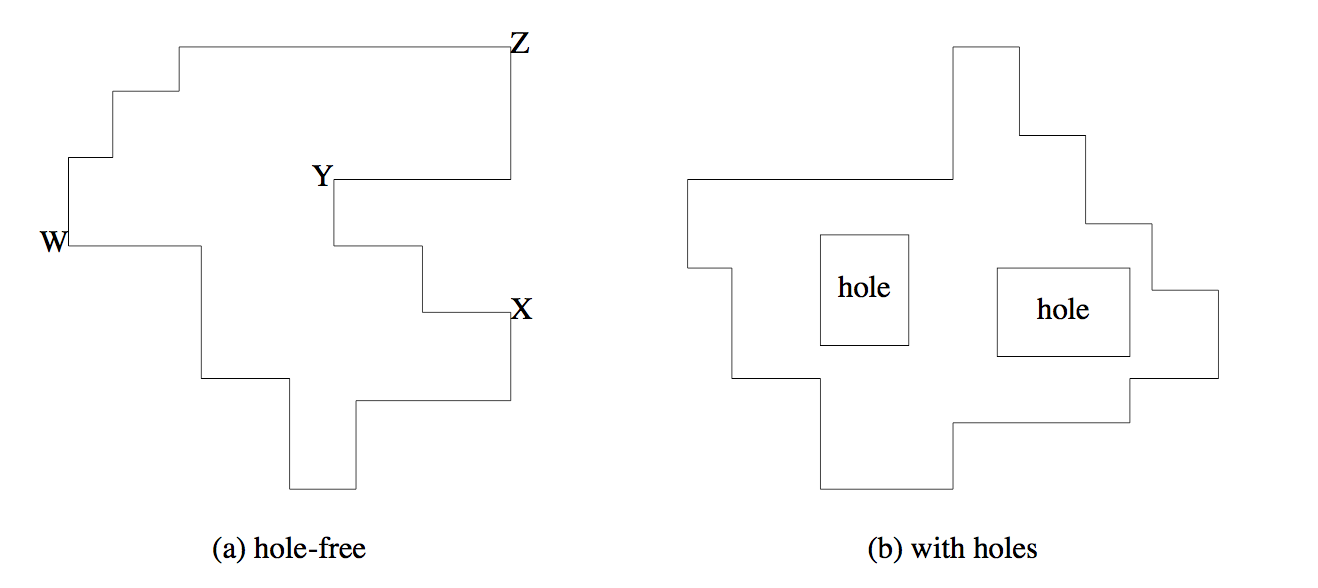
\includegraphics{Figures/fig1}}
    \caption{ Rectilinear Polygons [1]}
    \label{fig:Rect poly}
\end{figure}

A \textbf{\emph{minimal non-overlapping cover}} of a rectilinear polygon P is a rectangle partition of P that contains the fewest possible number of rectangles. The paper discusses a new complexity measure for the hole free rectilinear polygons. The paper defines the number of \emph{horizontal inversions, $k_{H}$} to be twice the minimum number of changes in horizontal motion while traveling around the polygon once. Similarly, the number of \emph{vertical inversions, $k_{V}$} to be twice the minimum number of changes in vertical motion while traveling around the polygon once.

The main complexity factor is \emph{k} which is given by
\begin{displaymath}
	 k = \min \{k_H, k_V\}
\end{displaymath}
This complexity measure covers a wide variety of polygons. The paper analysed 2869 polygons of which 85\% had \emph{k = 1} and 95\% had \emph{k $\leq$ 2}. Thus, for most practical reasons the \emph{O(kn)} algorithm is linear in time.
\\
\begin{figure}[h]
	\centering
	\scalebox{0.7}{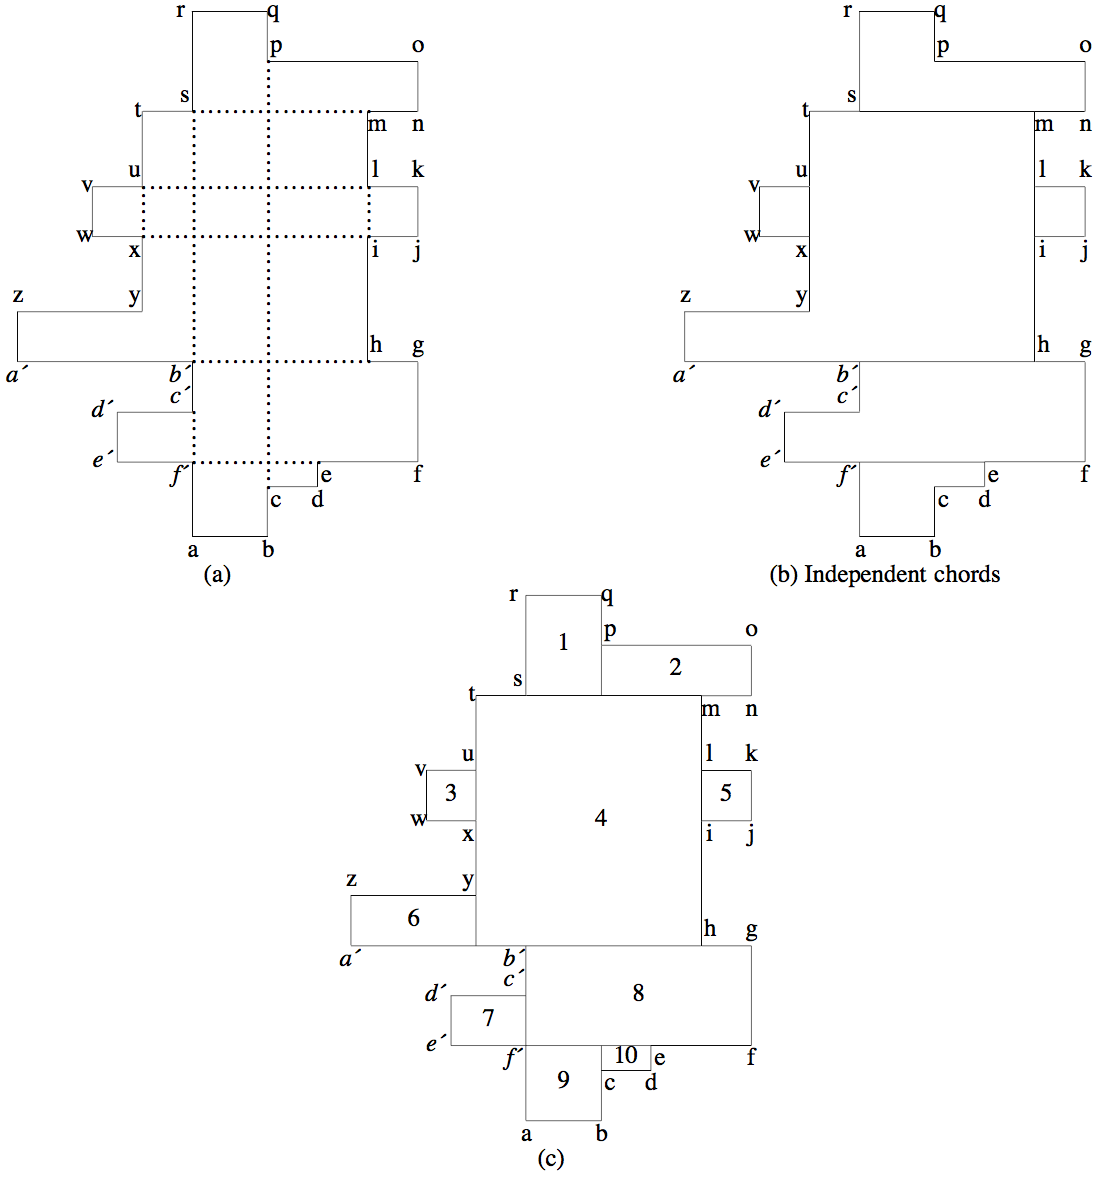
\includegraphics{Figures/fig2}}
	\caption{ Maximum Non-overlapping cover of a rectilinear polygon [1]}
	\label{fig:max cover}
\end{figure}
%----------------------------------------------------------------------------------------

\chapter{Definitions}
\label{Definitions}
\lhead{\emph{Definitions}}

\flushleft
\begin{enumerate}
	\item \textbf{Concave Vertices:} A vertex is said to be concave if the two edges intersecting at it makes an angle of $270^{\circ}$ with the interior of the polygon. For example, in Figure~\ref{fig:max cover}, the set of concave vertices  = \{c, h, i, l, m, p , s\}
	\item \textbf{Convex Vertices:} A vertex is said to be concave if the two edges intersecting at it makes an angle of $90^{\circ}$ with the interior of the polygon. For example, in Figure~\ref{fig:max cover}, the set of convex vertices = \{a, b, e, f\}
	\item \textbf{Chords: }A chord is a line joining any two co-horizontal concave vertices.
	\item \textbf{NEB(v): }Neighbourhood of a vertex v of a graph is defined as the set of all vertices, that have an edge incident from that vertex.
	\item \textbf{Convex Bipartite Graph: }A bipartite graph is said to be convex in V, if \forall{} v \in{}V, we can write it as a closed interval of the form [FIRST(v), LAST(v)]. In a convex bipartite graph labeling is crucial and needs to be defined for all problems together.
\begin{figure}[h]
	\centering
	\scalebox{0.45}{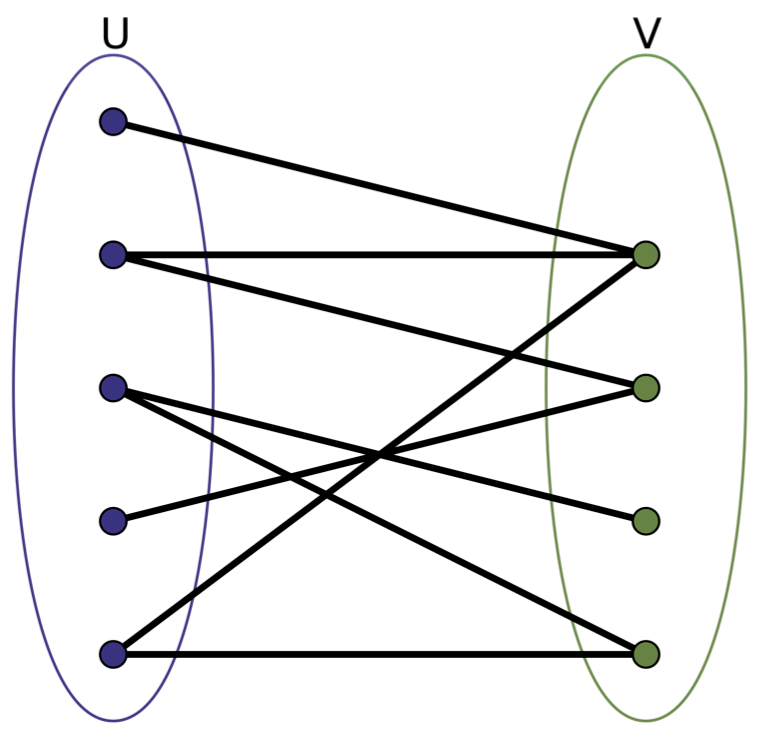
\includegraphics{Figures/fig3}}
	\caption{Convex Bipartite Graph on \emph{V} [4]}
	\label{fig:convex bipartite}
\end{figure}
  \item \textbf{Matchable vertex:} A vertex is matchable iff \exists y \in{} \emph{NEB(x)} such that,\emph{NEB(y)} \subseteq \emph{NEB(z)}, \forall z \in \emph{NEB(x)}.
  \item \textbf{Maximum Partition:} Partition of given rectillinear polygon into maximum number of non-overlapping rectangles.
  \item \textbf{Minimum Partition:} Partition of given rectillinear polygon into minimum number of non-overlapping rectangles, such that any two rectangles obtained , if merged will not form a rectangle.
\end{enumerate}

%----------------------------------------------------------------------------------------

\chapter{The Algorithm}
\label{The Algorithm}
\lhead{The Algorithm}
The algorithm is divided into multiple steps. The report reviews each step and the way of accepting input from the user, with a simple example.
\section{Method of Labelling the graph}
We take input as a rectilinear polygon from cursor keys, i.e., up($\uparrow$), left($\leftarrow$), and right ($\rightarrow$). As input is read, the pointer proceeds forward and draws a rectilinear polygon with its trail. The labelling of the vertices starts from $v_0$ to $v_{n-1}$, and $v_0 = v_n$, where n is the number of vertices in the polygon.

\begin{figure}[h]
	\centering
	\scalebox{0.5}{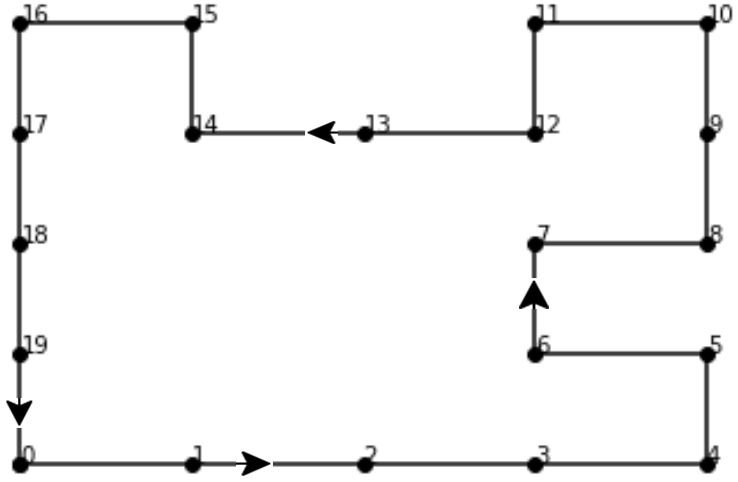
\includegraphics{Figures/fig6.png}}
	\caption{A Rectillinear polygon consisting of 20 vertices with direction of construction [5]}
	\label{fig:Rect poly example}
\end{figure}
\newpage
% --------------------------------------------------------
\section{INPUTS}
\textbf{G} = Rectilinear Graph \newline
\textbf{X} = Set of Abscissa of vertices \newline
\textbf{Y} = Set of Ordinates of vertices \newline
\textbf{Collinear\_Vertices} = Set of Collinear Vertices \newline
\textbf{Concave\_Vertices} = Set of Concave Vertices \newline
\textbf{Horizontal\_Chords} = Set of Horizontal Chords \newline
\textbf{Vertical\_Chords} = Set of Vertical Chords \newline

\underline{Important points to note}
\begin{enumerate}
\item Left and Right operations changes the direction the pointer faces.
\item Vertices that are induced after going forward consecutively. Although in the example, they are not explicitly shown,               but they do exist and at a distance of one unit from its previous vertex.
\item If the interior angle made by the two edges incident at this vertex is 270 degree.
\item Chords are lines joining two vertices which are not already part of the polygon.
\item As, the way of labelling is defined, there is unique labelling of each rectillinear polygon.
\end{enumerate}

\textbf{\emph{EXAMPLE:}}\\
In Figure~\ref{fig:Rect poly example}, the pointer is shown by an arrow. \newline
Total number of vertices = 20 \\
Collinear\_Vertices = [$v_{1}$, $v_{2}$, $v_{3}$, $v_{9}$, $v_{13}$, $v_{17}$, $v_{18}$, $v_{19}$] \\
Concave\_Vertices = [$v_{6}$, $v_{7}$, $v_{12}$, $v_{14}$] \\\*



\pagebreak
% --------------------------------------------------------

\section{Steps of Finding Maxiumum Partition}
\subsection{Step I}
\begin{lstlisting}
max_partition(G):
    for u in Concave_Vertices:
        for v in Concave_Vertices and v > u+1:
            if exists a chord joining v & u and ~exists another concave 
             vertex on chord joining v & u:
                if chord is horizontal: 
                    add (v, u) to Horizontal_Chords
                else if chord is vertical:
                    add (v, u) to Vertical_Chords
            else :
                loop_back
\end{lstlisting}
\textbf{Task Achieved:} All the edges that exist between \emph{any two concave vertices} are being added to their \emph{respectful categories}. \\
\textbf{\emph{EXAMPLE:}}\\
\begin{figure}[h]
  \centering
  \scalebox{0.5}{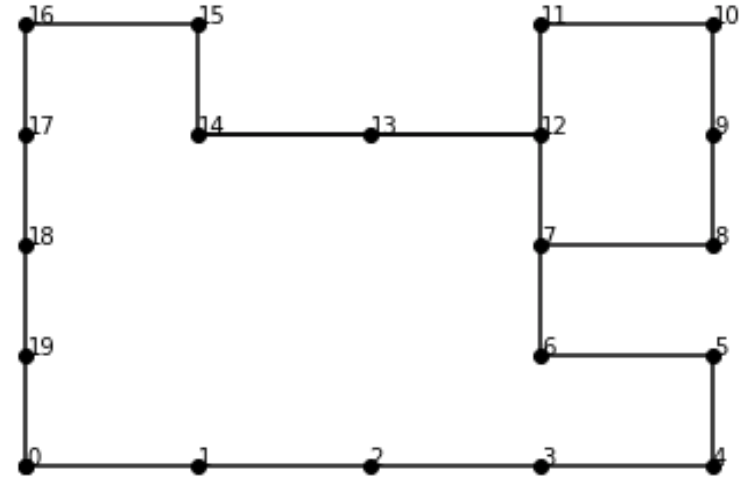
\includegraphics{Figures/fig5.png}}
\end{figure}

Horizontal\_Chords = \phi \\
Vertical\_chords = [($v_7$, $v_{12}$)] \\
\underline{Explanation:}
\textbf{u $>$ v :}Comparison between two vertices is done on the basis of their respective vertex indices. \
Here \textbf{v-u} should be greater than unity, because this assures the vertex v is not consecutive to u and has a higher index than u. Thus, iteration through each pair of vertex is done only once, making it more efficient. 

In the above code, we iterate through all (concave vertex, concave vertex') pairs, and check for existence of vertical and horizontal chords, that are not intersected by any other vertex.
We observe that, $v_7$ and $v_{12}$ are the only two concave vertices and between whom, there exists a vertical chord. Therefore, it is added to the set of \emph{Vertical\_Chords}. Also, there does not exist any horizontal chord between any two concave vertices and therefore, set of \emph{Horizontal\_Chords} is empty. \\

%----------------------------------------------------------
\subsection{Step II} % (fold)
\label{sub:step_2}
\begin{lstlisting}
 for u in Collinear_Vertices:
      for v in Concave_Vertices:
          if exists a chord joining v & u and ~exists another concave 
              or collinear vertex on chord joining v & u:
              if chord is horizontal:
                  add (v, u) to Horizontal_Chords
              else if chord is vertical:
                  add (v, u) to Vertical_Chords
          else :
              loop_back
\end{lstlisting}
\textbf{Task Achieved:} All the chords between \emph{collinear vertices and concave vertices} are being added to their \emph{respective categories}. 

\begin{figure}[h]
  \centering
  \scalebox{0.5}{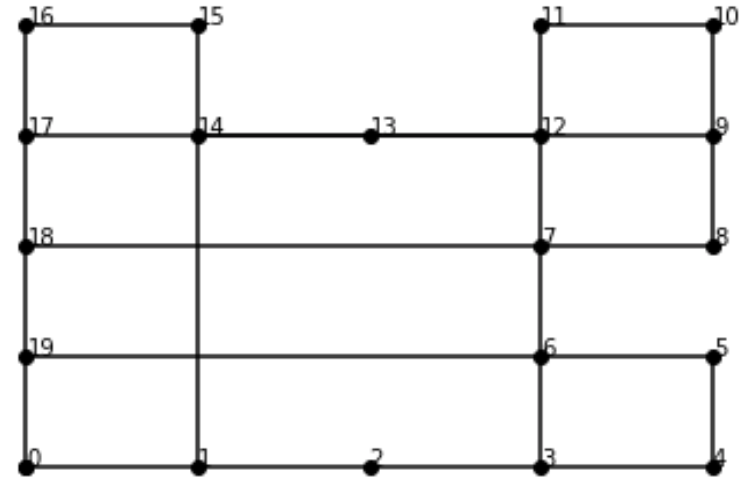
\includegraphics{Figures/fig4.png}}
\end{figure}

\emph{Horizontal\_Chords} =  [($v_{9}$, $v_{12}$), ($v_{17}$, $v_{14}$), ($v_{18}$, $v_{7}$), ($v_{19}$, $v_{6}$)] \\
\emph{Vertical\_Chords} =  [($v_{7}$, $v_{12}$), ($v_{1}$, $v_{4}$), ($v_{3}$, $v_{6}$)] 

\underline{Explanation}:
In the above code, we iterate through all (collinear vertex, concave vertex) pairs, and check for existence of vertical and horizontal chords between them, that are not intersected by any other vertex. \
If any chord is found, it is added to set of \emph{Vertical\_Chords or Horizontal\_Chords}, depending on its orientation. 

%----------------------------------------------------------
\subsection{Step III}

Thus, we have found all the chords, and only need to plot them now.

\begin{lstlisting}
    plot(X,Y)
    plot(Horizontal_Chords)
    plot(Vertical_Chords)
    display(plot)
\end{lstlisting}

\begin{figure}[h]
  \centering
  \scalebox{0.5}{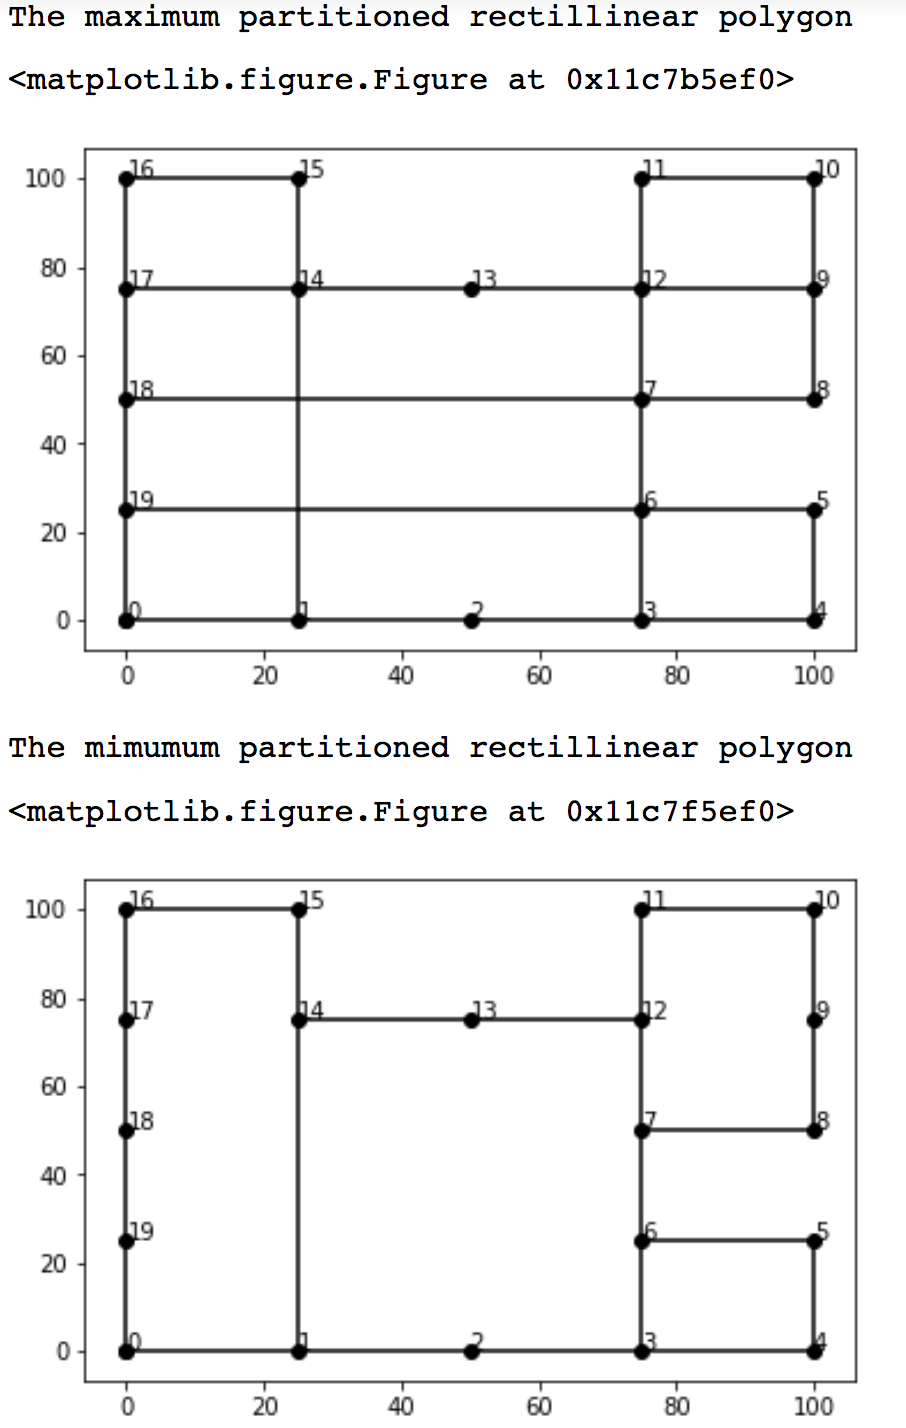
\includegraphics{Figures/fig7.png}}
\end{figure}
%----------------------------------------------------------

\subsection{Step IV}

Now we have found the maximum partition, but to find the minimum partition the following needs to be done
\begin{enumerate}
  \item Find a maximum independent set of chords (i.e., a maximum cardinality set of independent chords).
  \item Draw the chords in this maximum independent set. This partitions the polygon into smaller rectilinear polygons.
\end{enumerate}
%----------------------------------------------------------
\pagebreak
\subsection{Step V}
From each of the concave vertices from which a chord was not drawn in \emph{Step IV} draw a maximum length vertical line that is wholly within the smaller rectilinear polygon created in \emph{Step III} that contains this vertex.

%----------------------------------------------------------

\subsection{Step VI}

Thus, we have found all the chords, and only need to plot them now.
\begin{lstlisting}
    plot(X,Y)
    plot(Horizontal_Chords)
    plot(Vertical_Chords)
    plot(Nearest_Partial_Chords)
    display(plot)
\end{lstlisting}
%----------------------------------------------------------
\pagebreak

\section {Test Cases}

\textbf{INPUT 1}

\begin{figure}[h]
  \centering
  \scalebox{0.45}{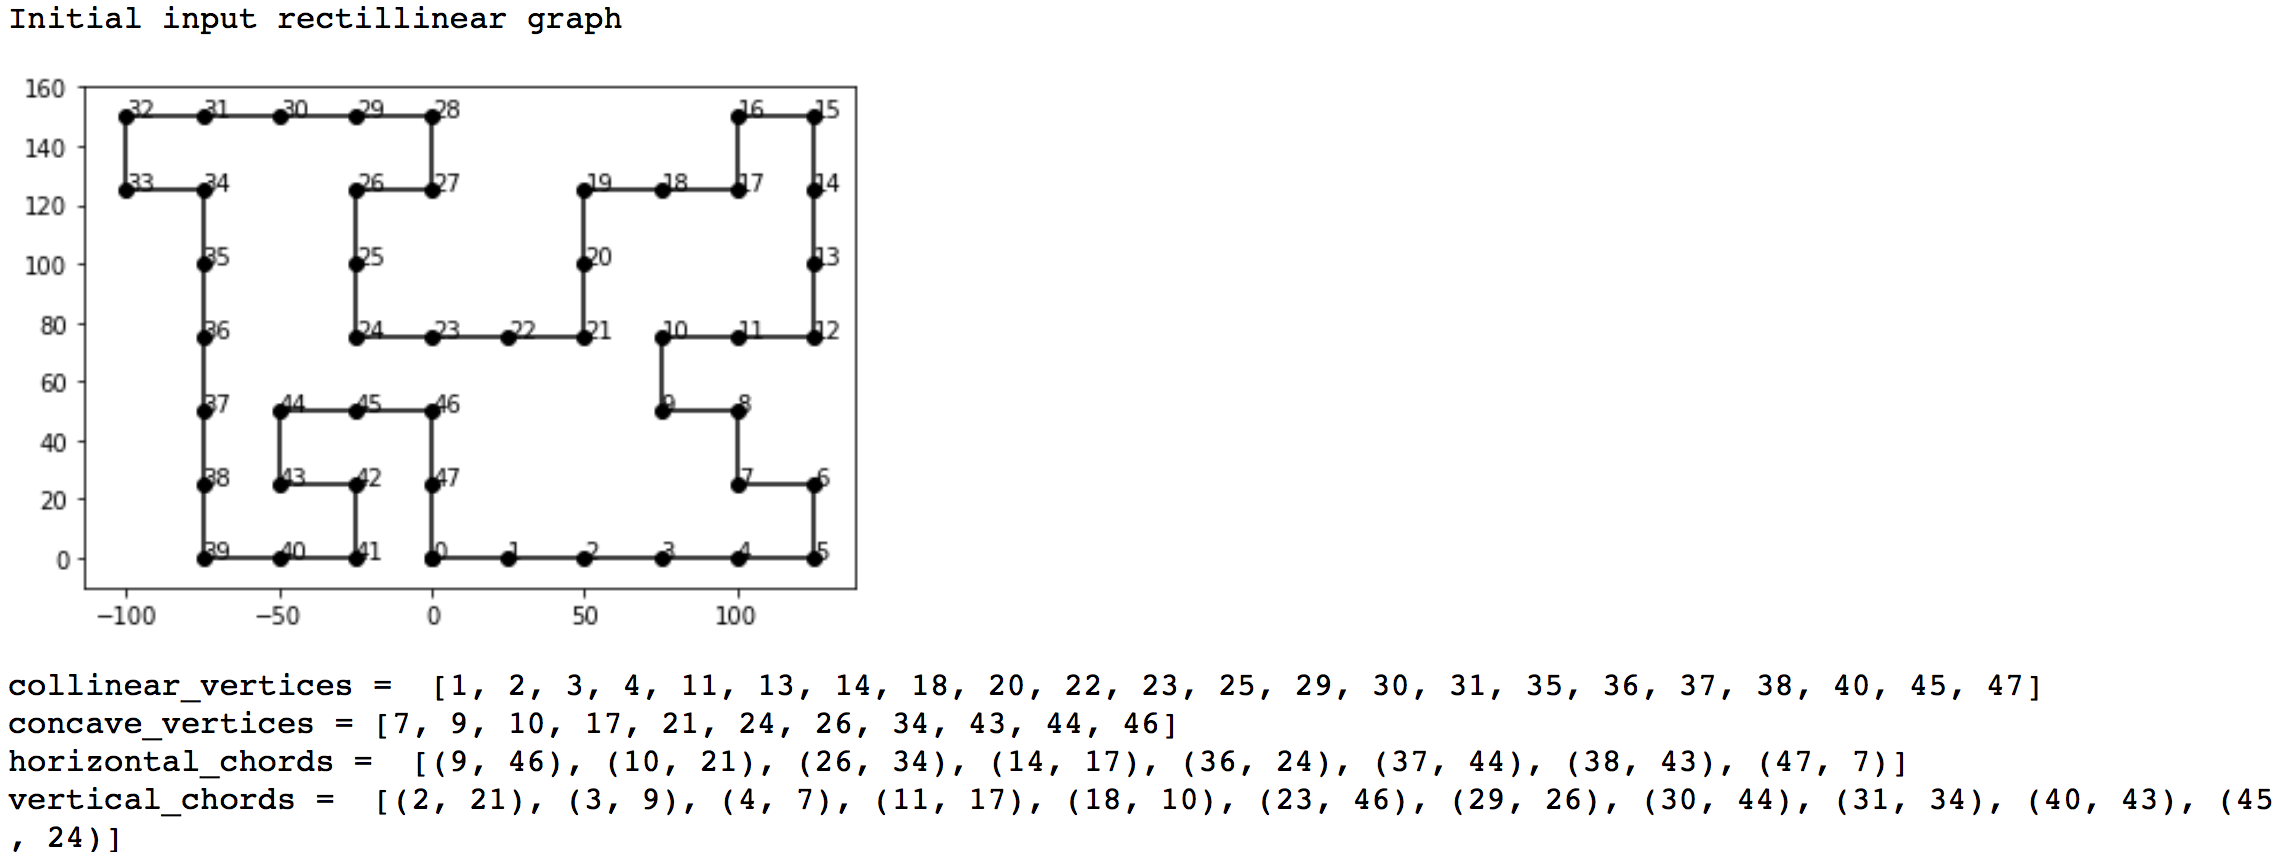
\includegraphics{Figures/t11.png}}
\end{figure}

\textbf{OUTPUT 1} 

\begin{figure}[h]
  \flushleft
  \scalebox{0.5}{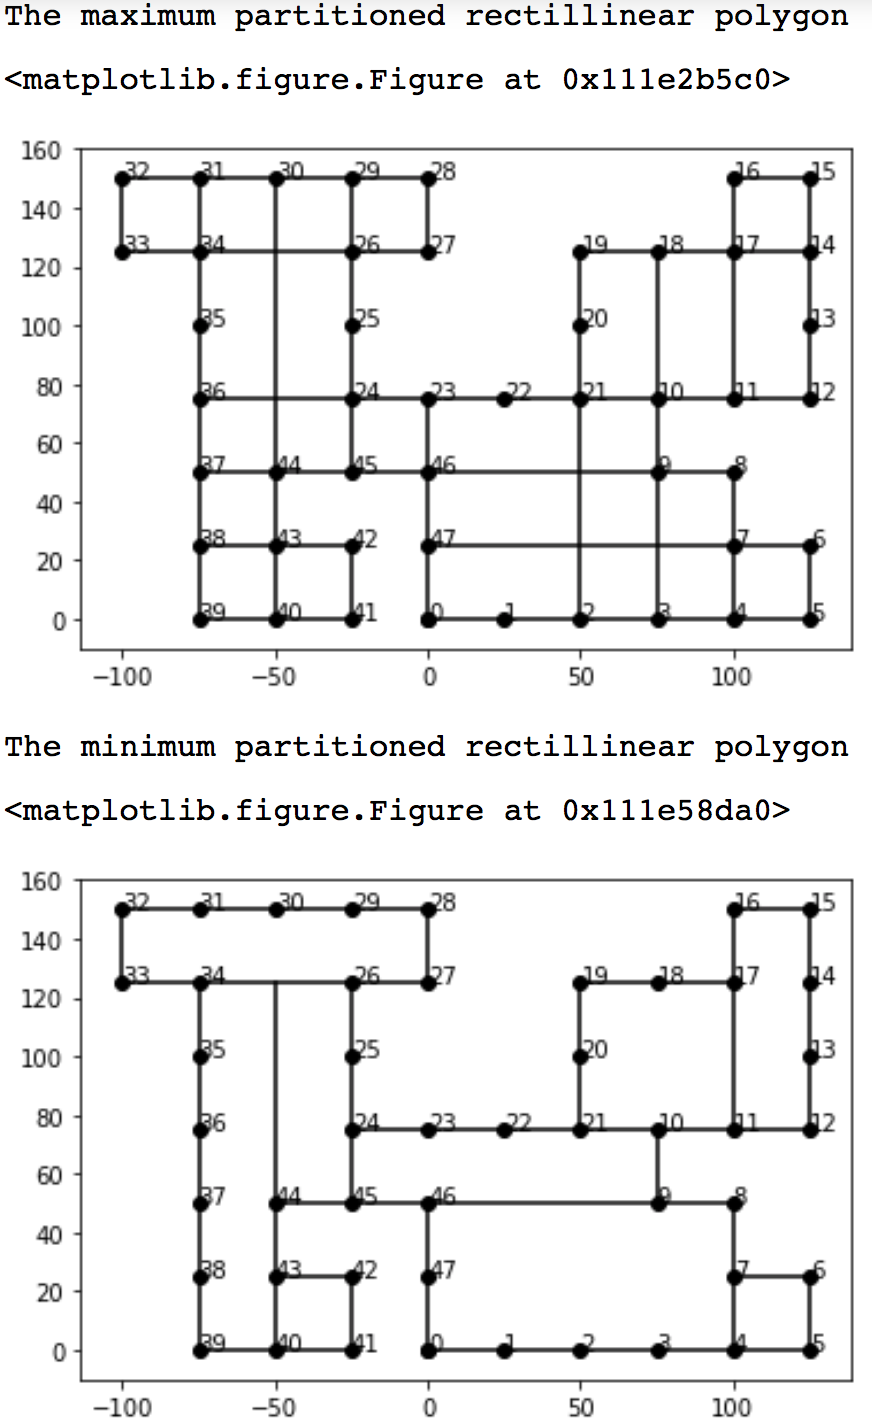
\includegraphics{Figures/t12.png}}
\end{figure}

\pagebreak
\textbf{INPUT 2}

\begin{figure}[h]
  \centering
  \scalebox{0.45}{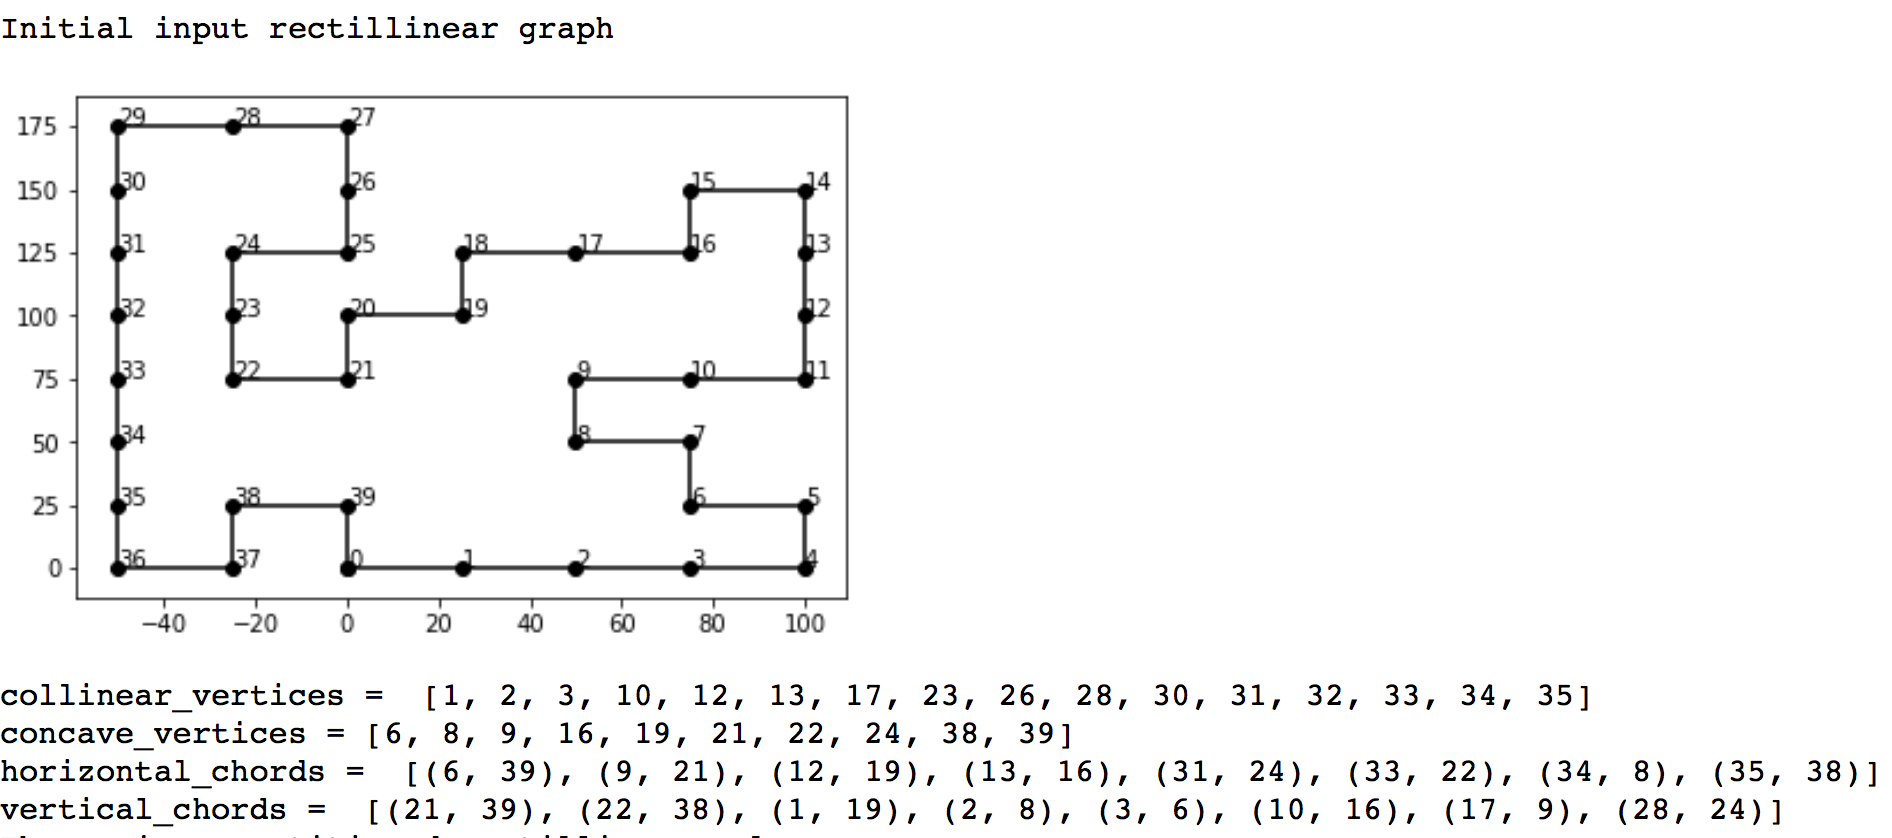
\includegraphics{Figures/t21.png}}
\end{figure}

\textbf{OUTPUT 2} 

\begin{figure}[h]
  \flushleft
  \scalebox{0.5}{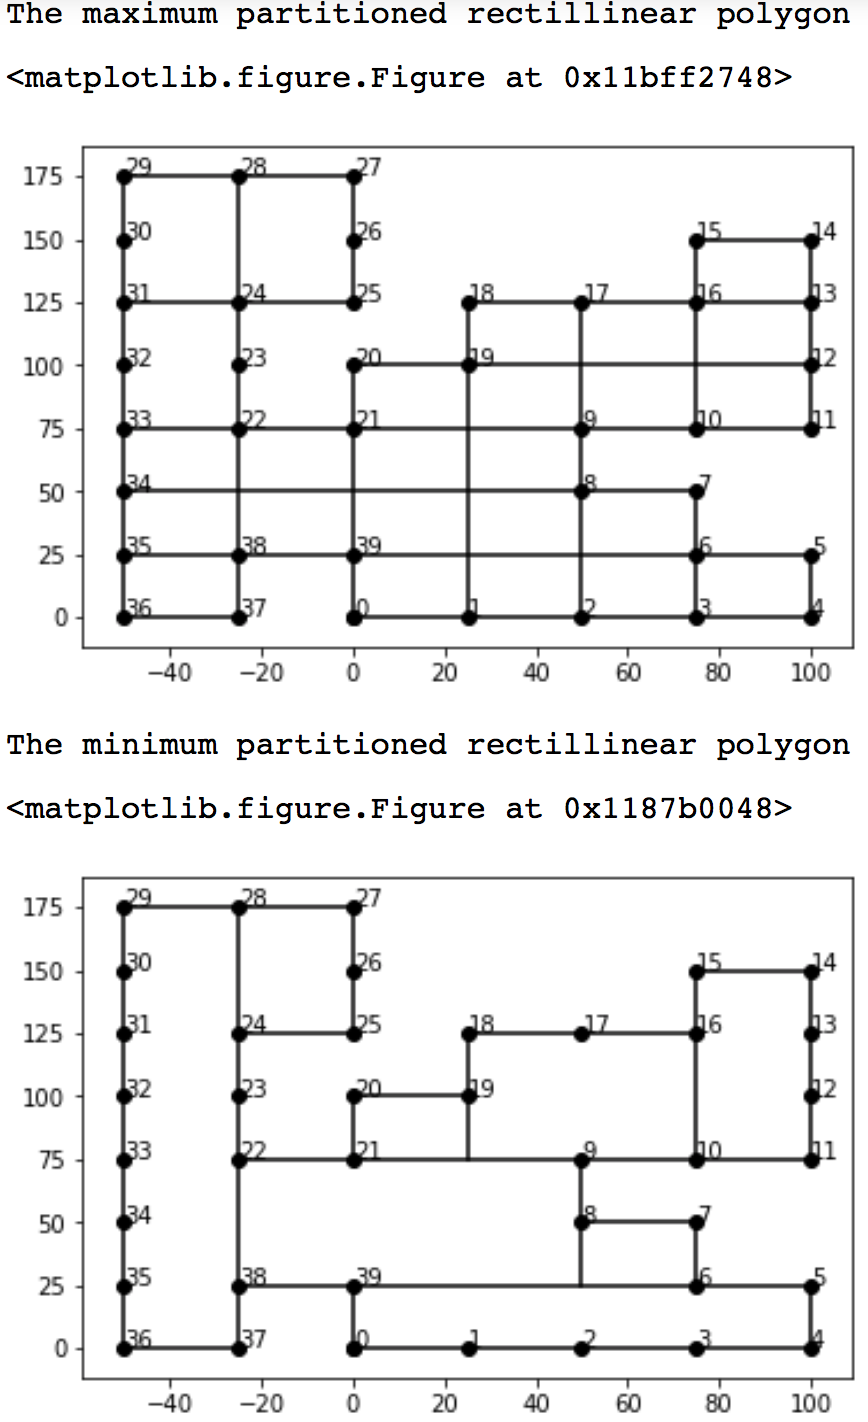
\includegraphics{Figures/t22.png}}
\end{figure}

\pagebreak
\textbf{INPUT 3}

\begin{figure}[h]
  \centering
  \scalebox{0.45}{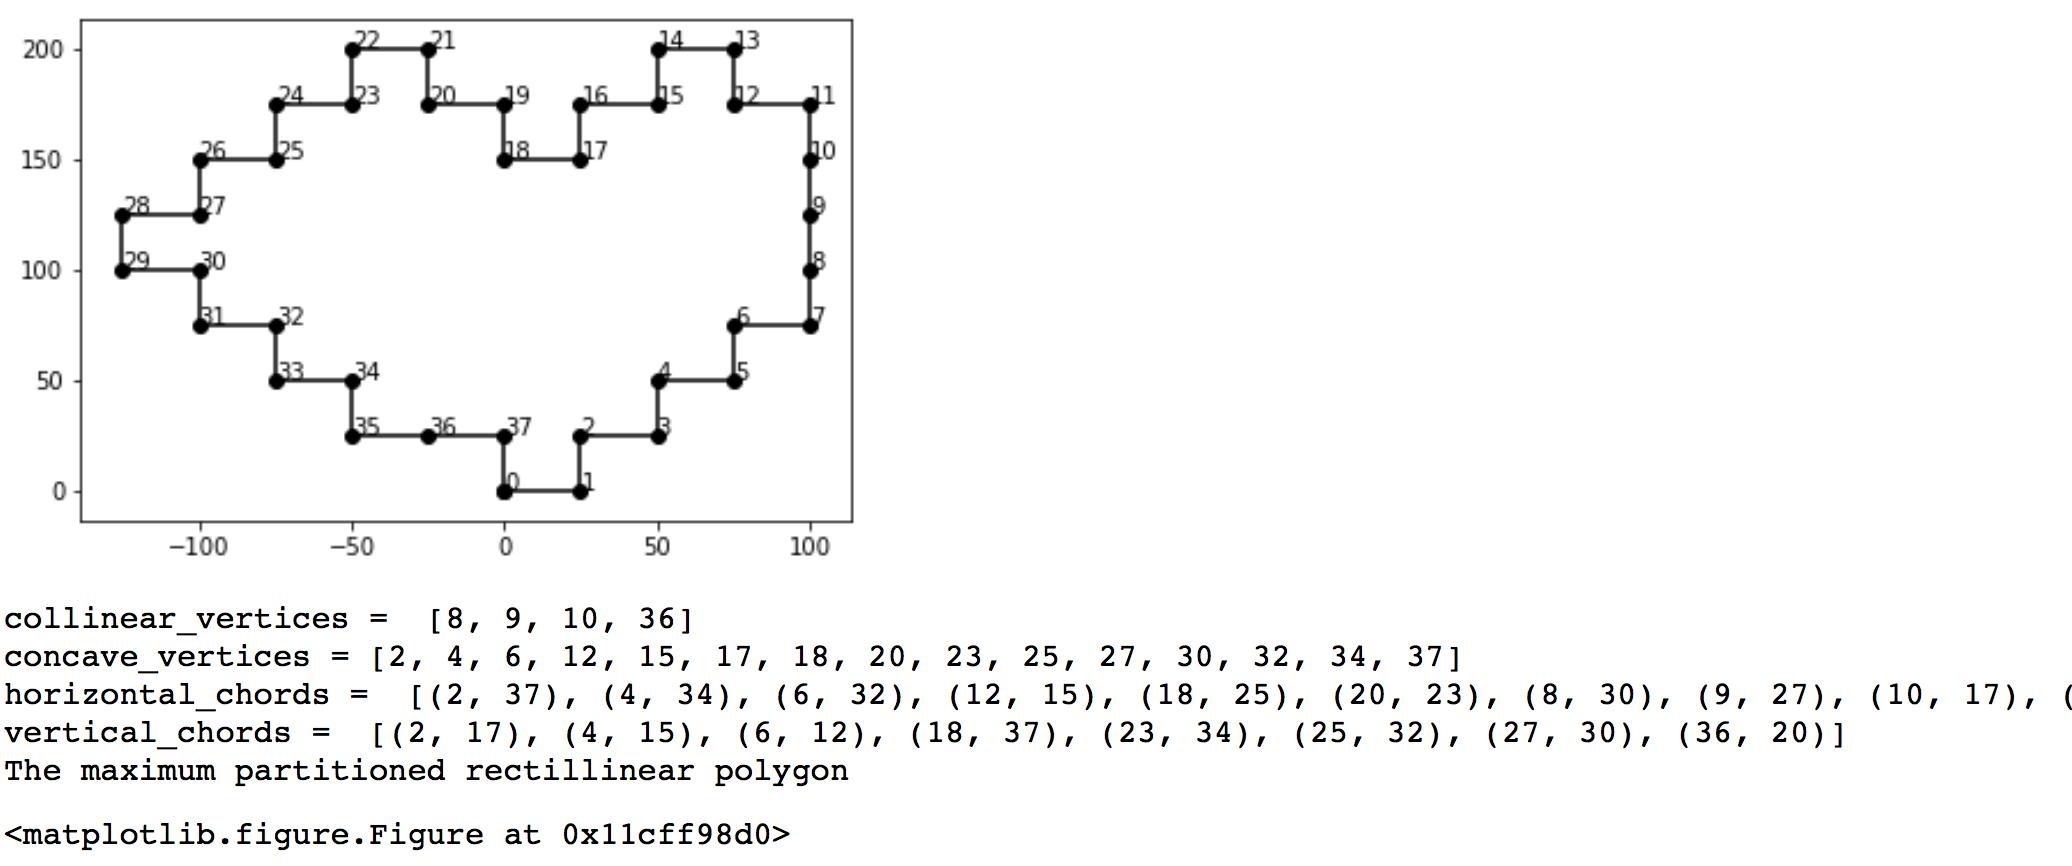
\includegraphics{Figures/t31.png}}
\end{figure}

\textbf{OUTPUT 3} 

\begin{figure}[h]
  \flushleft
  \scalebox{0.5}{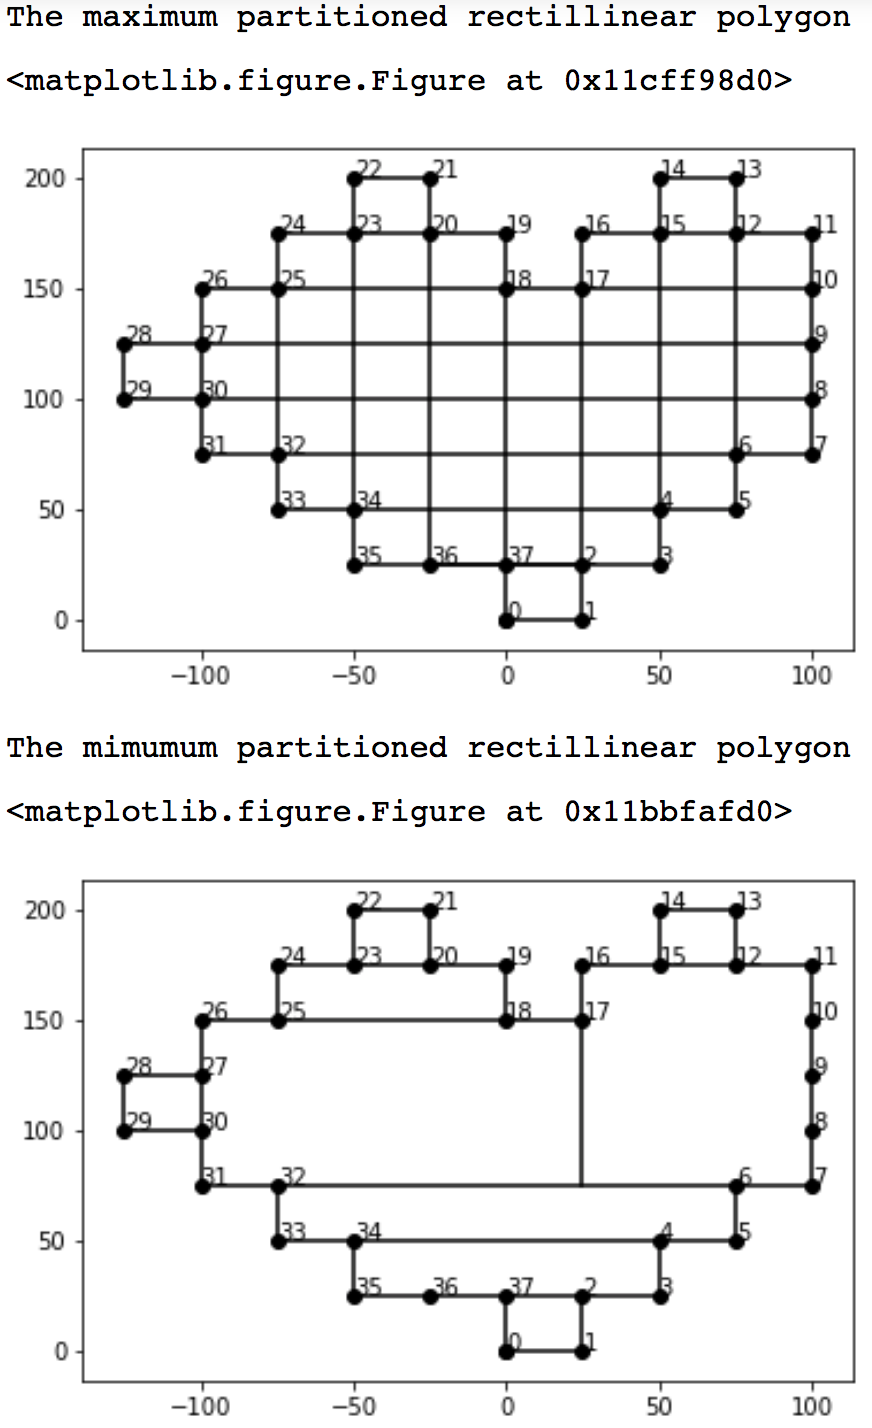
\includegraphics{Figures/t32.png}}
\end{figure}

\pagebreak
\textbf{INPUT 4}

\begin{figure}[h]
  \centering
  \scalebox{0.45}{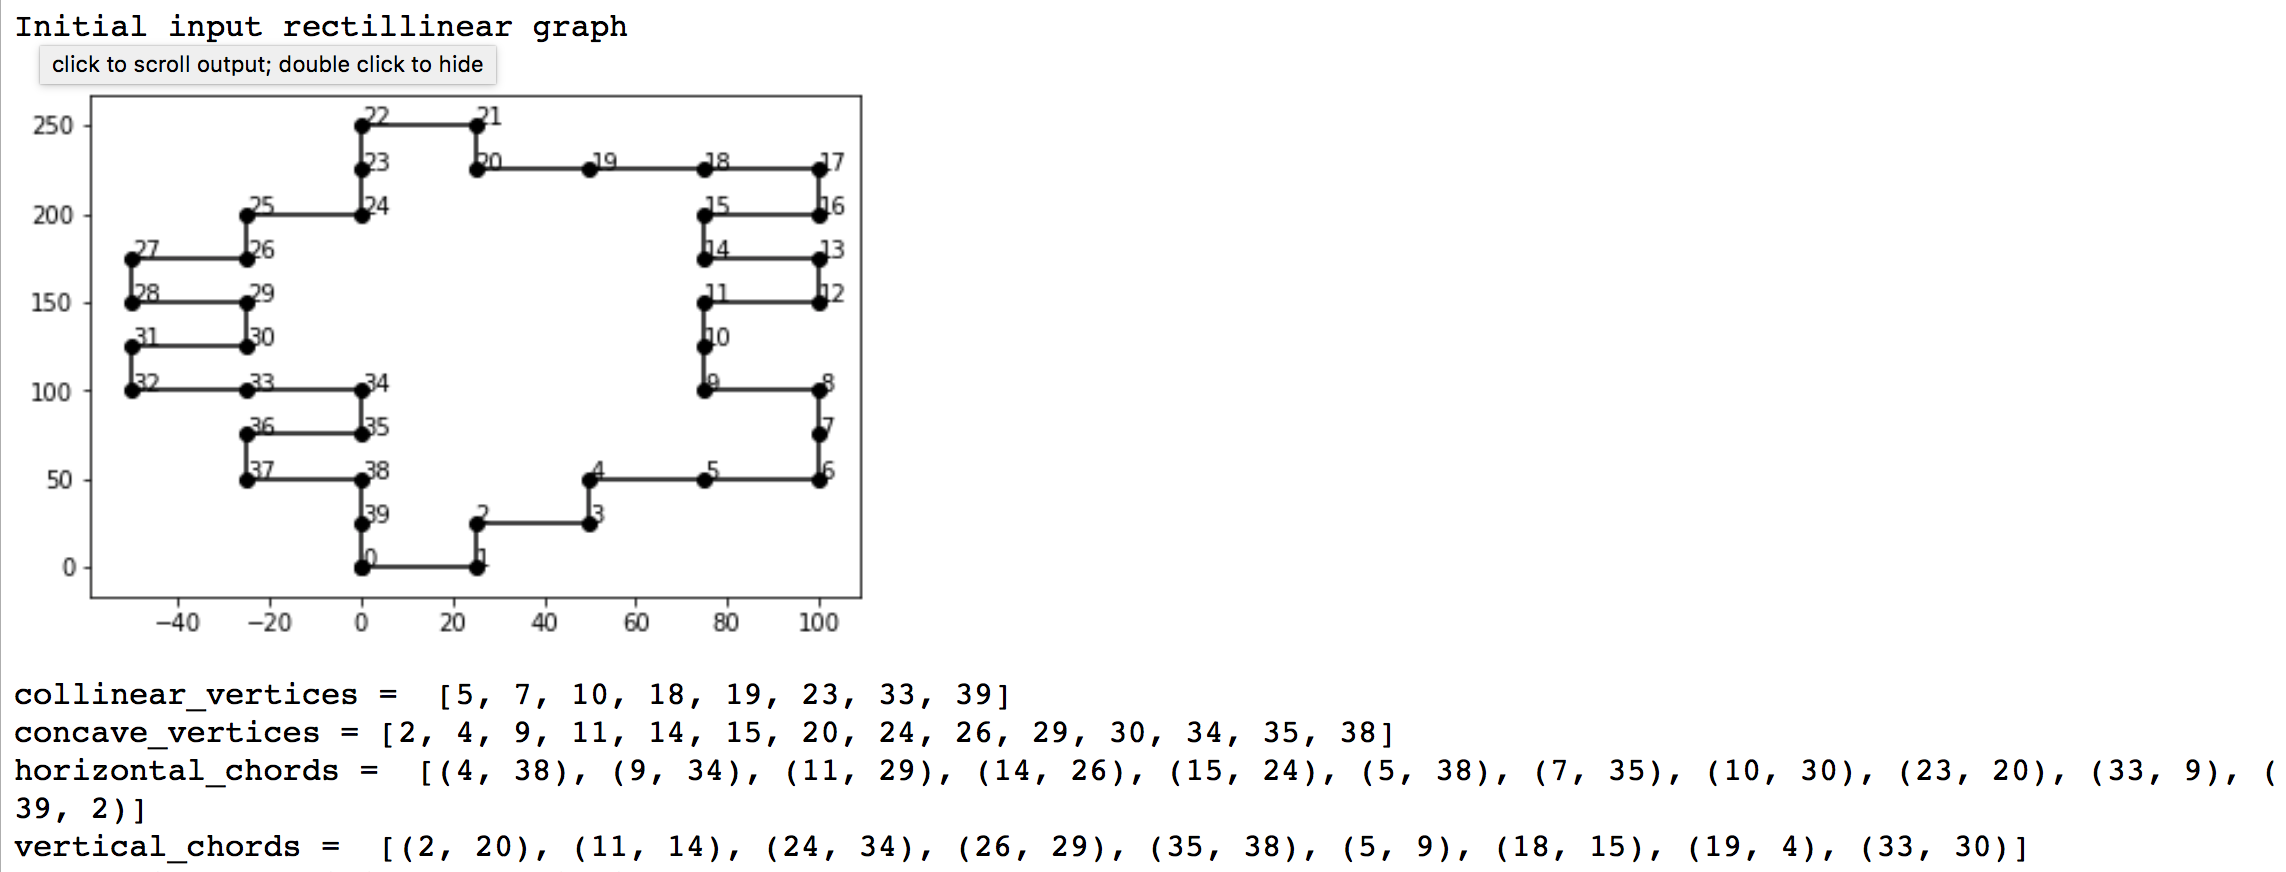
\includegraphics{Figures/t41.png}}
\end{figure}

\textbf{OUTPUT 4} 

\begin{figure}[h]
  \flushleft
  \scalebox{0.5}{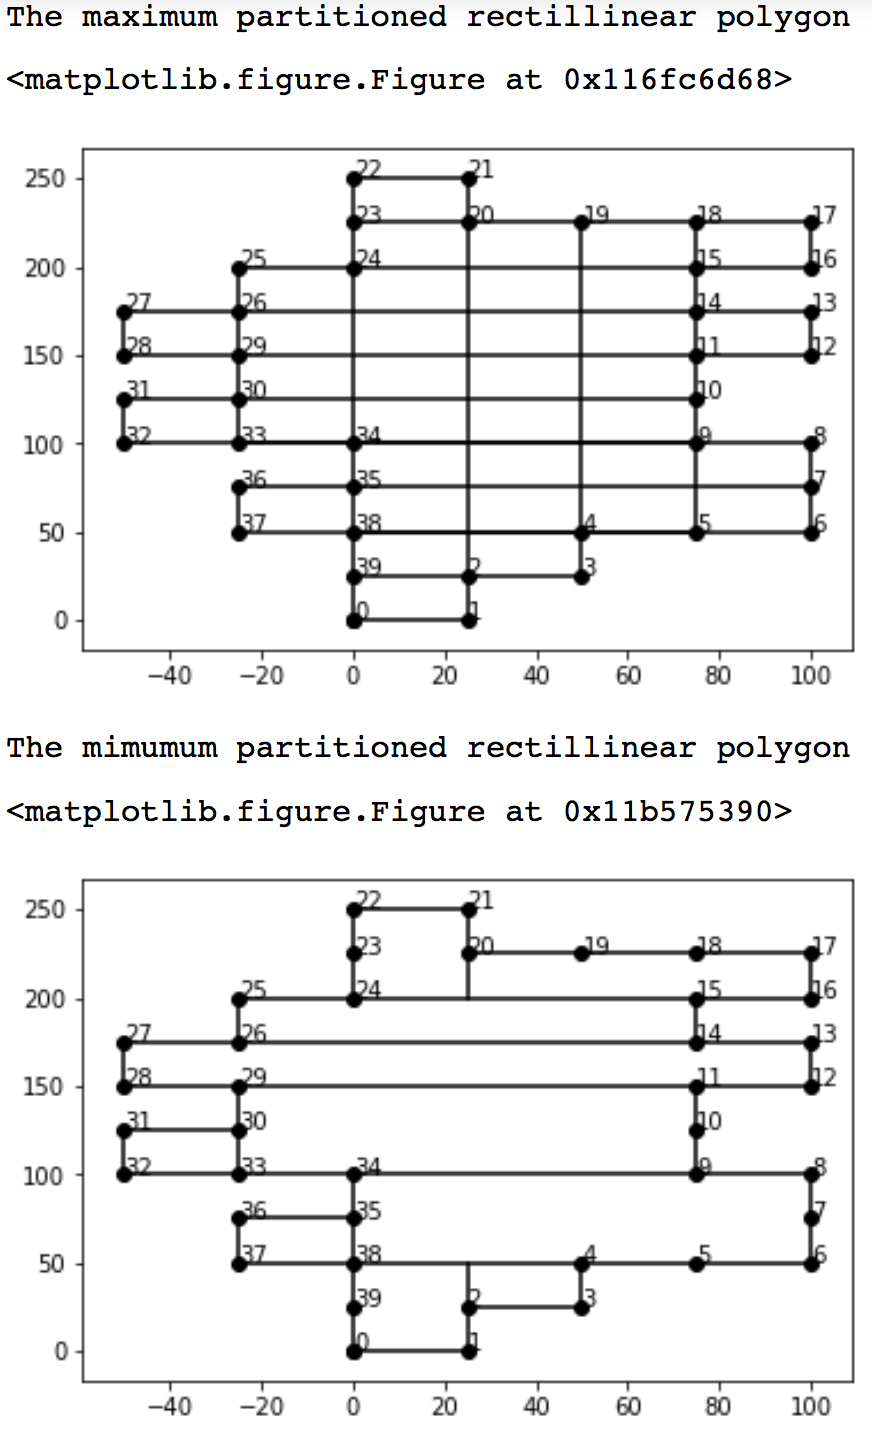
\includegraphics{Figures/t42.png}}
\end{figure}
%---------------------------------------------------

\chapter{Conclusion}
\label{Conclusion}
\lhead{Conclusion}

The algorithm reviewed does not give unique solutions, as the maximum independent set is not itself unique. Since, the horizontal and vertical sets of chords themselves make up two different set of maximum independent set of chords, if the number of horizontal chords and vertical chords are equal. Also there can be other maximum independent set of chords.

My future work will involve working on problems related to applications of graph theory, involving similar but more complicated and self-motivated problems.

Thus, this implementation and design with the newest tools will help architects, in preparing their own architectural arrangements, according to their choice.
%\input{Chapters/Chapter2}
%\input{Chapters/Chapter3}
%\input{Chapters/Chapter4}
%\input{Chapters/Chapter5}
%\input{Chapters/Chapter6}
%\input{Chapters/Chapter7}

%-------------------------------------------------------------------------------
%	THESIS CONTENT - APPENDICES
%-------------------------------------------------------------------------------

\addtocontents{toc}{\vspace{2em}} % Add a gap in the Contents, for aesthetics

\appendix % Cue to tell LaTeX that the following 'chapters' are Appendices

% Include the appendices of the thesis as separate files from the Appendices
% folder
% Uncomment the lines as you write the Appendices

% Appendix A

\chapter{Working Code in Python} % Main appendix title

\label{AppendixA} % For referencing this appendix elsewhere, use \ref{AppendixA}

\lhead{\emph{Working Code in Python}} % This is for the header on each page - perhaps a shortened title
\begin{lstlisting}
'Please make sure that the INPUT is A CLOSED RECTILINEAR POLYGON,'
'CONSTRUCTED WHILE GOING IN ANTI-CLOCKWISE ONLY'
# importing libraries
import networkx as nx
import turtle
import matplotlib.pyplot as plt
import warnings
from networkx.algorithms import bipartite
import math

warnings.filterwarnings("ignore")
# declaration list
wn = turtle.Screen()
# a turtle called gopu 
gopu = turtle.Turtle() 
# co-ordinate points
x = [] 
y = []
# vertex-type := rectilinear = -1; convex = 0; concave = 1 
vertex_type = [] 
# store the bipartite graph of chords
G = nx.Graph()
# the line below can be commented if one needs animation
gopu.speed(0)
# starts recording keys being pressed
gopu.begin_poly()

# Event handlers
stride = 25
# Up  = up() - vertex to be deleted = -1
def up():
    vertex_type.append(-1)
    gopu.forward(stride)
 
# left = left() ; make vertex - convex = 0
def left():
    vertex_type.append(0)
    gopu.setheading(gopu.heading()+90)
    gopu.forward(stride)
 
# right = right() ; make vertex - concave = 1
def right():
    vertex_type.append(1)
    gopu.setheading(gopu.heading()-90)
    gopu.forward(stride)
 
# back = back() -- doing undo is allowed only once.
def back():
    vertex_type.pop()
    gopu.undo()

# quits the screen and outputs the plots the partitioned polygon
def partition_polygon():
    # closing the screen
    wn.bye()
    # stopped recording the polygon
    gopu.end_poly()
    p = gopu.get_poly()
    p = list(p)
    compute_partition(p)  
    
'''
The movements of the turtle are recorded and the rectilinear polygon thus 
obtained is converted into bipartite graph of chords
'''
def compute_partition(p):
    # p now contains the list of coordinates of vertices
    # last one is same as the origin
    # and the origin is always going to be a convex vertex
    p.pop()
    vertex_type[0] = 0
    
    # x and y contain list of x and y coordinates respectively
    for i,j in p:
        x.append(i)
        y.append(j)

    # this is done as there are some very small errors in recording the 
    # position by the turtle library
    for i in range(len(x)):
        x[i] = int(x[i])
        y[i] = int(y[i])

    for i in range(len(x)):
        if x[i] % stride != 0:
            x[i] += (stride - x[i] % stride)
        if y[i] % stride != 0:
            y[i] += (stride - y[i] % stride)

    # separating concave and collinear vertices
    collinear_vertices = [i for i,val in enumerate(vertex_type) if val == -1]
    concave_vertices = [i for i,val in enumerate(vertex_type) if val == 1]
    
    # finding the chords inside the polygon
    horizontal_chords = []
    vertical_chords = []

    # middles is used because, there are cases when there is a chord between vertices
    # and they intersect with external chords, hence if there is any vertex in between 
    # two vertices then skip that chord. 
    for i in range(len(concave_vertices)):
        for j in range(i+1,len(concave_vertices)):
            if concave_vertices[j] != concave_vertices[i] + 1:
                middles = []
                if y[concave_vertices[i]] == y[concave_vertices[j]]:
                    for k in range(len(x)):
                        if y[concave_vertices[i]] == y[k] and (x[concave_vertices[i]] < x[k] and x[concave_vertices[j]] > x[k] \
                                                              or x[concave_vertices[i]] > x[k] and x[concave_vertices[j]] < x[k]):
                            middles.append(k)
                    if len(middles) == 0:
                        horizontal_chords.append((concave_vertices[i],concave_vertices[j]))
                middles = []
                if x[concave_vertices[i]] == x[concave_vertices[j]]:
                    for k in range(len(x)):
                        if x[concave_vertices[i]] == x[k] and (y[concave_vertices[i]] < y[k] and y[concave_vertices[j]] > y[k] \
                                                              or y[concave_vertices[i]] > y[k] and y[concave_vertices[j]] < y[k]):
                            middles.append(k)
                    if len(middles) == 0:
                        vertical_chords.append((concave_vertices[i],concave_vertices[j]))
            

    temp_hori = horizontal_chords[:]
    temp_verti = vertical_chords[:]

    for i in range(len(collinear_vertices)):
        for j in range(len(concave_vertices)):
            middles = []
            if y[collinear_vertices[i]] == y[concave_vertices[j]]:
                if collinear_vertices[i] < concave_vertices[j]:
                    for k in range(len(x)):
                        if y[k] == y[collinear_vertices[i]] and (x[k] < x[concave_vertices[j]] \
                            and x[k] > x[collinear_vertices[i]] or x[k] > x[concave_vertices[j]] \
                            and x[k] < x[collinear_vertices[i]]):
                            middles.append(k)
                    if collinear_vertices[i]+1 == concave_vertices[j]:
                        middles.append(0)
                else:
                    for k in range(len(x)):
                        if y[k] == y[collinear_vertices[i]] and (x[k] > x[concave_vertices[j]] \
                            and x[k] < x[collinear_vertices[i]] or x[k] < x[concave_vertices[j]] \
                            and x[k] > x[collinear_vertices[i]]):
                            middles.append(k)
                    if collinear_vertices[i] == concave_vertices[j]+1:
                        middles.append(0)
                if len(middles) == 0:
                    horizontal_chords.append((collinear_vertices[i],concave_vertices[j]))
            middles = []
            if x[collinear_vertices[i]] == x[concave_vertices[j]]:
                if collinear_vertices[i] < concave_vertices[j]:
                    for k in range(len(x)):
                        if x[k] == x[collinear_vertices[i]] and (y[k] < y[concave_vertices[j]] \
                            and y[k] > y[collinear_vertices[i]] or y[k] > y[concave_vertices[j]] \
                            and y[k] < y[collinear_vertices[i]]):
                            middles.append(k)
                    if collinear_vertices[i]+1 == concave_vertices[j]:
                        middles.append(0)
                else:
                    for k in range(len(x)):
                        if x[k] == x[collinear_vertices[i]] and (y[k] > y[concave_vertices[j]] \
                            and y[k] < y[collinear_vertices[i]] or y[k] < y[concave_vertices[j]] \
                            and y[k] > y[collinear_vertices[i]]):
                            middles.append(k)
                    if collinear_vertices[i] == concave_vertices[j]+1:
                        middles.append(0)
                if len(middles) == 0:
                    vertical_chords.append((collinear_vertices[i],concave_vertices[j]))    
    # displaying all attributes and important parameters involved
    # plotting the initial input given
    print ("Initial input rectillinear graph")
    fig, ax = plt.subplots()
    ax.plot(x+[0], y+[0], color='black')
    ax.scatter(x+[0], y+[0], color='black')
    for i in range(len(x)):
        ax.annotate(i, (x[i],y[i]))
    plt.show()
    plt.clf()
    
    print("collinear_vertices = ", collinear_vertices)
    print("concave_vertices =", concave_vertices)
    print("horizontal_chords = " ,horizontal_chords)
    print("vertical_chords = ",vertical_chords)
    
    # drawing the maximum partitioned polygon 
    print("The maximum partitioned rectillinear polygon")
    fig, ax = plt.subplots()
    ax.plot(x+[0], y+[0], color='black')
    ax.scatter(x+[0], y+[0], color='black')
    for i in range(len(x)):
        ax.annotate(i, (x[i],y[i]))
    for i,j in horizontal_chords:
        ax.plot([x[i],x[j]],[y[i],y[j]],color='black')
    for i,j in vertical_chords:
        ax.plot([x[i],x[j]],[y[i],y[j]],color='black')
    plt.show()
    plt.clf()
    # MAXIMUM PARTITION CODE ENDS ---------------------------------

    # MINIMUM PARTITION CODE STARTS -------------------------------
    horizontal_chords = temp_hori[:]
    vertical_chords = temp_verti[:]

    # Creating a bipartite graph from the set of chords
    for i,h in enumerate(horizontal_chords):
        y1 = y[h[0]]
        x1 = min(x[h[0]] ,x[h[1]] )
        x2 = max(x[h[0]] ,x[h[1]])
        G.add_node(i, bipartite=1)
        for j,v in enumerate(vertical_chords):
            x3 = x[v[0]]
            y3 = min(y[v[0]],y[v[1]])
            y4 = max(y[v[0]],y[v[1]])
            G.add_node(j + len(horizontal_chords),bipartite=0)
            if x1 <= x3 and x3 <=x2 and y3 <= y1 and y1 <= y4:    
                G.add_edge(i, j + len(horizontal_chords))
    
    if len(horizontal_chords) == 0:
        for j,v in enumerate(vertical_chords):
            x3 = x[v[0]]
            y3 = min(y[v[0]],y[v[1]])
            y4 = max(y[v[0]],y[v[1]])
            G.add_node(j,bipartite=0)
    
    # finding the maximum matching of the bipartite graph, G.
    M = nx.Graph()
    maximum_matching = nx.bipartite.maximum_matching(G)
    maximum_matching_list = []
    for i,j in maximum_matching.items():
        maximum_matching_list += [(i,j)]
    M.add_edges_from(maximum_matching_list)
    maximum_matching = M.edges()
    # breaking up into two sets
    H, V = bipartite.sets(G)
    free_vertices = []
    for u in H:
        temp = []
        for v in V:
            if (u,v) in maximum_matching or (v,u) in maximum_matching:
                temp += [v]
        if len(temp) == 0:
            free_vertices += [u]
    for u in V:
        temp = []
        for v in H:
            if (u,v) in maximum_matching or (v,u) in maximum_matching:
                temp += [v]
        if len(temp) == 0:
            free_vertices += [u]
            
    # finding the maximum independent set
    max_independent = []
    while len(free_vertices) != 0 or len(maximum_matching) != 0:
        if len(free_vertices) != 0 :
            u = free_vertices.pop()
            max_independent += [u]
        else:
            u, v = maximum_matching.pop()
            G.remove_edge(u,v)
            max_independent += [u]

        for v in G.neighbors(u):
            G.remove_edge(u, v)
            for h in G.nodes():
                if (v,h) in maximum_matching:
                    maximum_matching.remove((v,h))
                    free_vertices += [h]
                if (h,v) in maximum_matching:
                    maximum_matching.remove((h,v))
                    free_vertices += [h]

    
    # drawing the partitioned polygon 
    independent_chords = []
    for i in max_independent:
        if (i >= len(horizontal_chords)):
            independent_chords += [vertical_chords[i-len(horizontal_chords)]]
        else:
            independent_chords += [horizontal_chords[i]]
    unmatched_concave_vertices = [i for i in concave_vertices]
    for i,j in independent_chords:
        if i in unmatched_concave_vertices:
            unmatched_concave_vertices.remove(i)
        if j in unmatched_concave_vertices:
            unmatched_concave_vertices.remove(j)
    
    nearest_chord = []
    for i in unmatched_concave_vertices:
        dist = 0
        nearest_distance = math.inf
        for j in max_independent:
            if j < len(horizontal_chords):
                temp1, temp2 = horizontal_chords[j]
                if abs(y[i] - y[temp1]) < nearest_distance and \
                (x[i] <= x[temp1] and x[i] >= x[temp2] or x[i] >= x[temp1] and x[i] <= x[temp2]) \
                and abs(temp1 - i) != 1 and abs(temp2 - i) != 1:
                    middles = []
                    for u in range(len(x)):
                        if x[i] == x[u] and (y[i] < y[u] and y[u] < y[temp1] or y[temp1] < y[u] and y[u] < y[i]):
                            middles.append(u)
                    if len(middles) == 0:
                        nearest_distance = abs(y[i] - y[temp1])
                        dist = y[temp1] - y[i]

        if nearest_distance != math.inf:
            nearest_chord.append((i,dist)) 
        else:
            for k in collinear_vertices:
                if x[k] == x[i] and abs(y[k] - y[i]) < nearest_distance and abs(k-i) != 1:
                    middles = []
                    for u in range(len(x)):
                        if x[i] == x[u] and (y[i] < y[u] and y[u] < y[k] or y[k] < y[u] and y[u] < y[i]):
                            middles.append(u)
                    if len(middles) == 0:
                        nearest_distance = abs(y[i] - y[k])
                        dist = y[k] - y[i]
            nearest_chord.append((i,dist)) 
     
    print("The minimum partitioned rectillinear polygon")
    fig, ax = plt.subplots()
    ax.plot(x+[0], y+[0], color='black')
    ax.scatter(x+[0], y+[0], color='black')
    for i in range(len(x)):
        ax.annotate(i, (x[i],y[i]))
    for i,j in independent_chords:
        ax.plot([x[i],x[j]],[y[i],y[j]],color='black')
    for i,dist in nearest_chord:
        ax.plot([x[i],x[i]],[y[i], y[i]+dist],color='black')
    plt.show()
    # MAXIMUM PARTITION CODE ENDS
# Defining the keyboard keys function
wn.onkey(up, "Up")
wn.onkey(left, "Left")
wn.onkey(right, "Right")
wn.onkey(back, "Down")
wn.onkey(partition_polygon, "Escape")
wn.listen()
wn.mainloop()


\end{lstlisting}
%\input{Appendices/AppendixB}
%\input{Appendices/AppendixC}

\addtocontents{toc}{\vspace{2em}} % Add a gap in the Contents, for aesthetics

\backmatter

%-------------------------------------------------------------------------------
%	BIBLIOGRAPHY
%-------------------------------------------------------------------------------
\chapter{References}
\label{References}

\lhead{\emph{References}} % Change the page header to say "Bibliography"

\begin{enumerate}
	\item Wu, San-Yuan, and Sartaj Sahni. "Fast algorithms to partition simple rectilinear polygons." VLSI Design 1.3 (1994): 193-215.
	\item  \href{http://networkx.github.io/}{Networkx Library(Accessed on: 23^{rd} March, 2017)}
	\item \href{http://www.python.org/ }{Python(Accessed on: 23^{rd} March, 2017)}
	\item \href{http://en.wikipedia.org/}{Wikipedia (Accessed on: 23^{rd} February, 2017)}
	\item \href{https://github.com/mittalgovind/Polygon-Partition}{Author's Github Repository}
\end{enumerate}
\end{document}
